\Chapter{Backend Dokumentáció}

\Section{Projekt inicializálás}

A projetket a Spring Boot Initializr segítségével hoztam létre.

\begin{figure}[h]
\centering
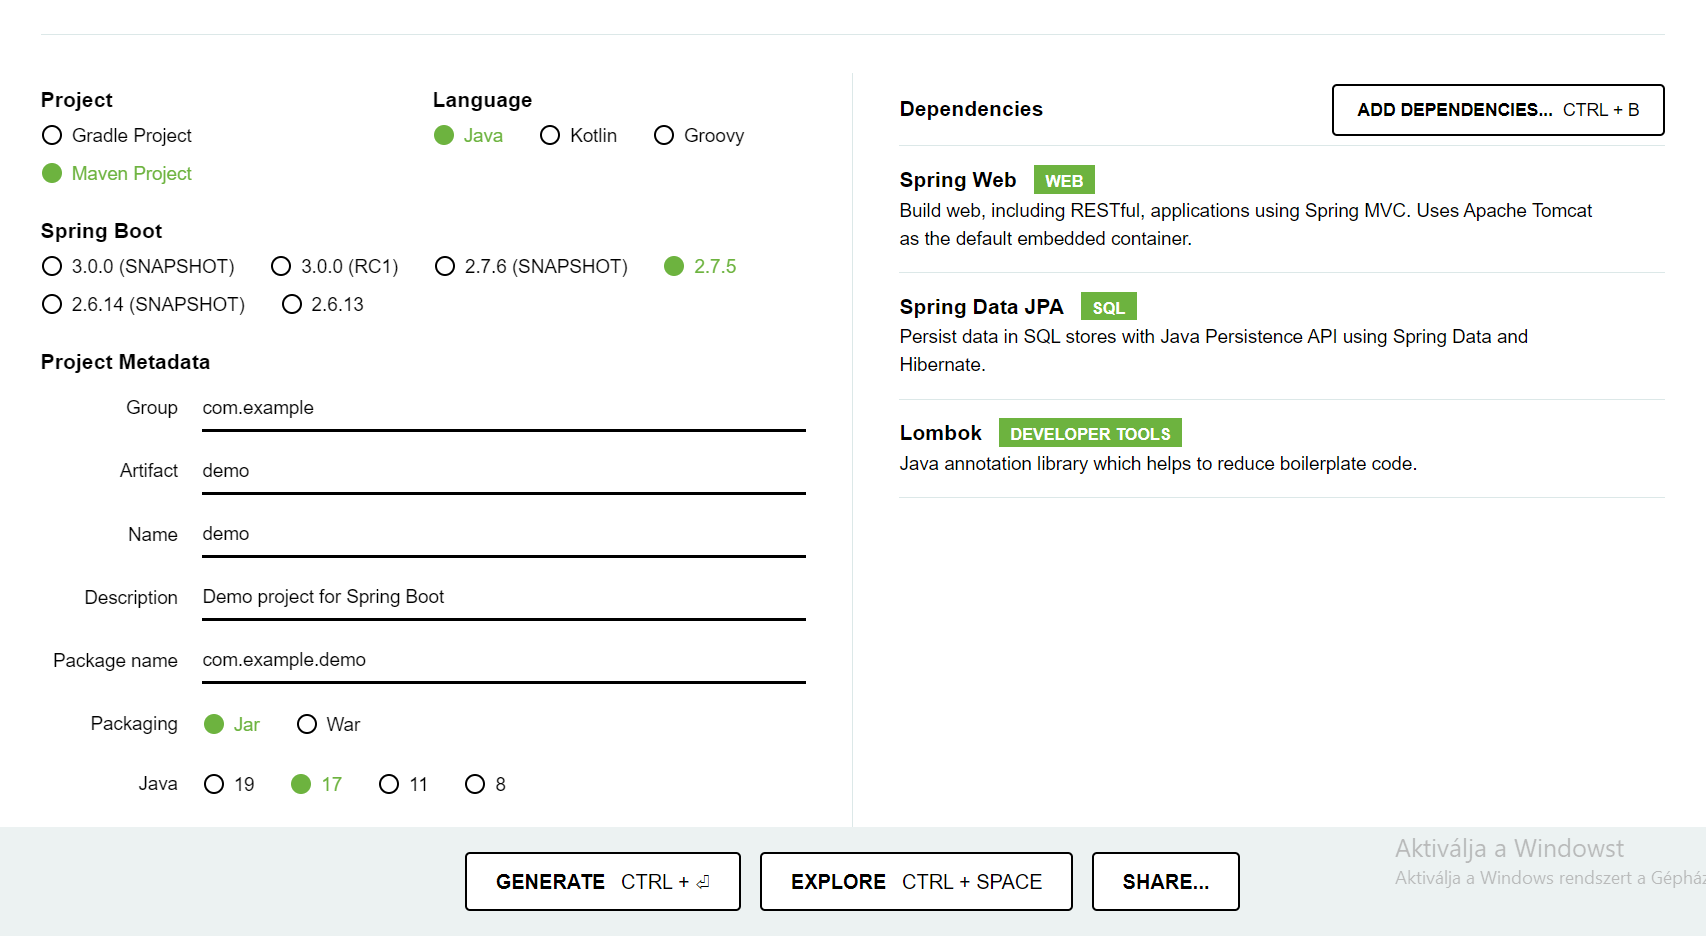
\includegraphics[scale=0.37]{images/Spring_init.png}
\caption{Spring Boot Initializr\cite{SpringInit}}
\label{fig:Spring_Boot_Initializr}
\end{figure}

Ahogy az ábrán is látszik ki lehet választani, hogy milyen típusú projekt legyen milyen nyelven szeretnénk elkészíteni, a Spring Boot verzióját, metaadatokat milyen Java verzióra szeretnénk fejleszteni.

Dependency-ket tudunk megadni. A létrehozáskor a Spring Web-et, a Spring Data JPA-t és a Lombokot adtam hozzá.

Dependency-k a pom.xml fájlban találhatóak meg. 

Mikor mindent kiválasztottunk a GENERATE gombra nyomva le is generálja ne-
künk az alap projektet.
\newpage
Elkészített projekt mappaszerkezete így néz ki:
\begin{figure}[h]
\centering
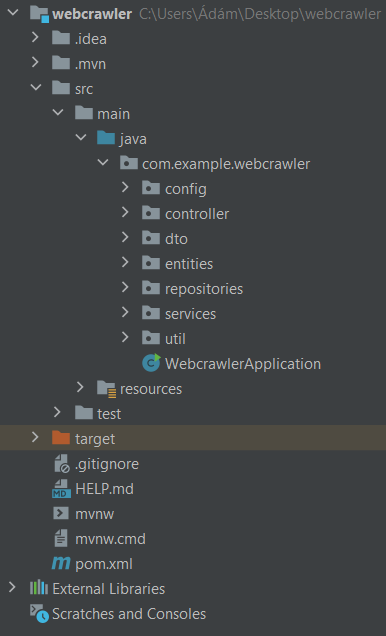
\includegraphics[scale=0.7]{images/Intelij-mappaszerkezet.png}
\caption{Intelij-mappaszerkezet}
\label{fig:Intelij-mappaszerkezet}
\end{figure}

Maga a szerver a http://localhost:8080/ címen fut.

\Section{Adatbázis léthrehozása} 

Első lépésben az Adatbázis létrehozásához 2 dependency-t kellett használnom amit a pom.xml fájlba kellett elhelyezni:
\begin{itemize}
\item spring-boot-starter-data-jpa
\item postgresql
\end{itemize}

Miután a behelyezés megtörtént az adatbázisunkat hozzá kell kapcsolni a szer-
verünkhöz ami az application.properties fájlban történik. Én PostgreSQL-t adatbázist használok az adatok tárolására és a kapcsolat így jön létre a DB és a szerver között:

\begin{java}
spring.datasource.url=jdbc:postgresql://localhost:5432/cardb
spring.datasource.username=postgres
spring.datasource.password=Password
spring.jpa.properties.hibernate.dialect= org.hibernate.dialect
.PostgreSQLDialect
spring.jpa.properties.hibernate.format_sql=true
\end{java}

Az Url az adatbázis szerver és maga az adatbázis eléréséhez szükséges. A szerver a 5432 porton fut és a cardb adatbázisra lesz szükségünk.
A username és password ahoz kell, hogy tudjuk magunkat hitelesíteni.

Következő lépésben létrehoztam a 3 adatbázis táblát(car,search-data,users)amihez létrehoztam mindegyikhez egy entity-t és egy repository-t.

Entity-n belül tudjuk, megadni, hogy a táblán belül milyen oszlopok legyenek és hogy mi legyen az elsődleges kulcs.

Példa egy Entity Java osztályra ami a users nevű táblát hozza létre:

\begin{java}
@Getter
@Setter
@NoArgsConstructor
@AllArgsConstructor
@Entity
@Table(name="users")
public class User {
    @Id
    @GeneratedValue(strategy = GenerationType.IDENTITY)
    @Column(name = "user_id")
    private int id;

    @Column(name = "login")
    private String login;

    @Column(name = "password")
    private String password;

    @Column(name = "authority")
    private String authority;
}
\end{java}

A Repository-ra azért van szükségünk hogy a szerverünk tudjon kommunikálni az adatbázissal, tehát hogy tudjon adatot lekérdezni vagy felvinni törölni vagy éppen módosítani és ehhez ki kell terjeszteni a JpaRepository osztályt ami tartalmaz alapvető műveleteket.

Példa egy Repository osztályra:

\begin{java}
@Repository
public interface UserRepository extends
			JpaRepository<User, Integer>
{

    List<User> deleteByLogin(String login);
    User findUserByLogin(String login);
}
\end{java}
\newpage

\Section{Autók lekérdezése az adatbázisba}

Az adatok megszerzéséhez WebCrawlert használok. Ami azt jelenti hogy az adatokat a weboldalak HTML-tartalmából gyűjtöm össze, tehát ehhez az egész weboldal felépítését át kell hozzá néznem mivel tag-ek vagy éppen cssQuerry-vel lehet egyes adatokat kinyerni. 

Én esetemben ez azért volt elég nehezen megoldható, mert arra is figyelni kellett, hogy vannak olyan autók a honlapon amik nem rendelkeznek az összes adattal azért ki kellett szűrni az olyan autókat amik úgymond hibásan vannak feltéve. 

Lent látható egy példa egy WebCrawler-re

\begin{figure}[h]
\centering
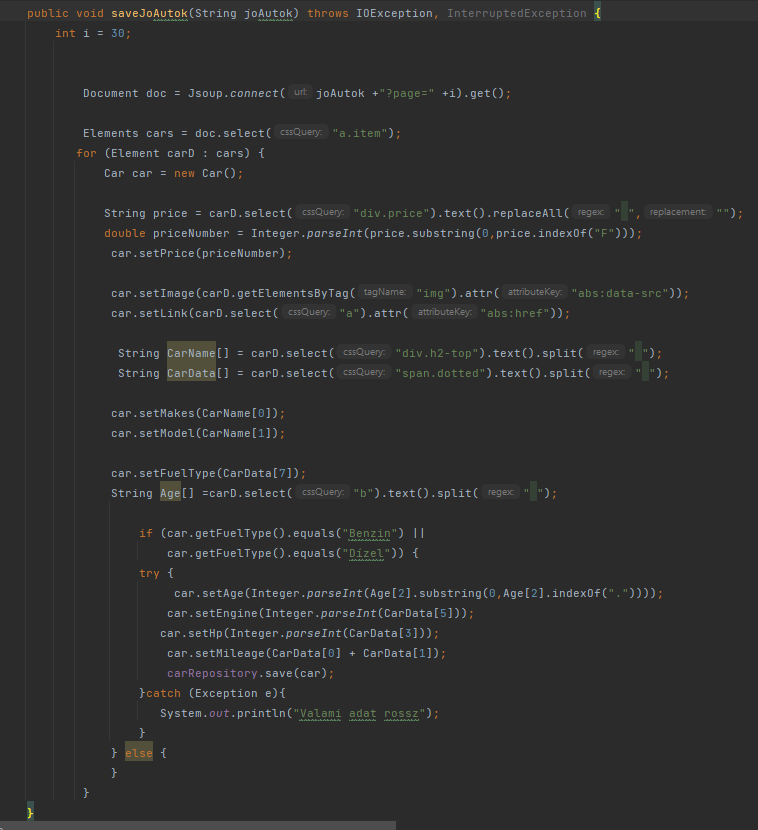
\includegraphics[scale=0.7]{images/JoAutok_WebCrawler.png}
\caption{JóAutók-WebCrawler}
\label{fig:JóAutók-WebCrawler}
\end{figure}

\Section{Autók lekérdezése az adatbázisból}

Ha valaki autókra szeretne keresni akkor a /get végpont hívódik meg ami Request-
Paramétereket vár ami más néven QuerryParaméter. Rengeteg paraméter kell egy ilyen lekérdezéshez amit opcionálisan ki is lehet hagyni így arra volt szükségem hogy dinamikus lekérdezést tudjak létrehozni amihez a Criteria API-t használom.

JPA Specification teszi azt lehetővé hogy dinamikus legyen a lekérdezés ami a Criteria API-ra épül, tehát nem kell minden adatnak szerepelnie benne vagy éppen úgy is működik ha nincsen benne szereplő kritérium hogy mi alapján kérdezze le az adatokat mert akkor az összeset lekérdezi az adatbázisból. A Predicate interfészével tudjuk összekötni a Querry-nket a vizsgálat után.

\begin{figure}[h]
\centering
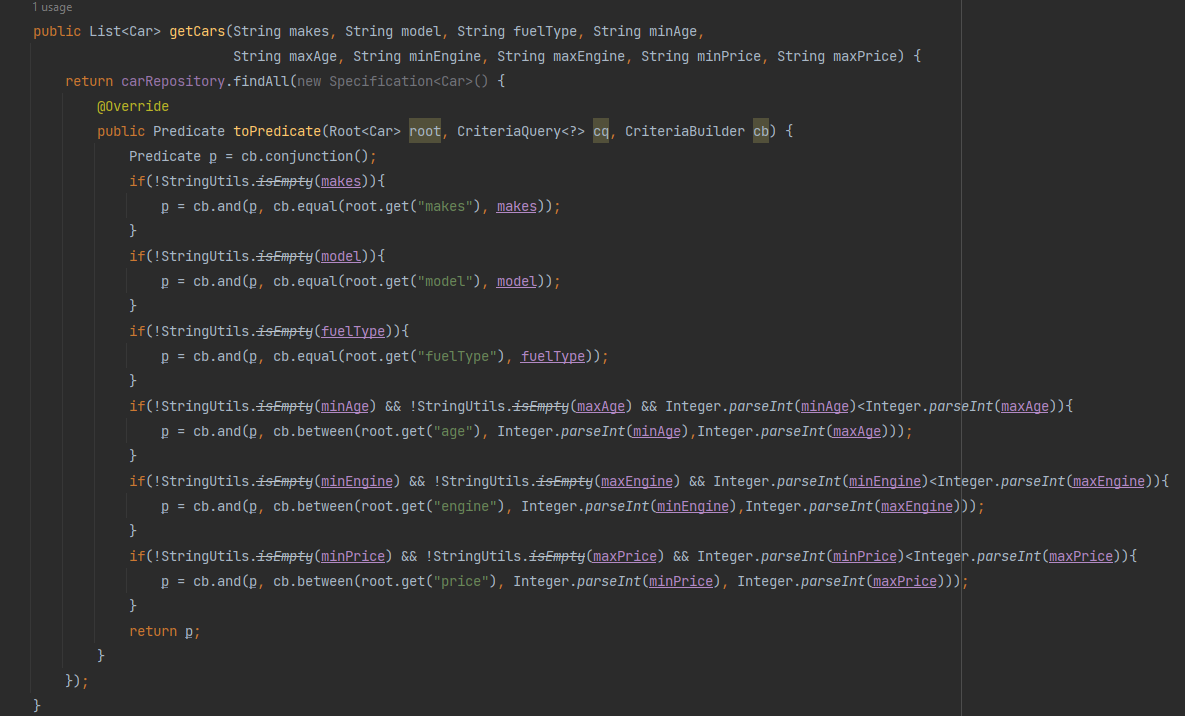
\includegraphics[scale=0.6]{images/Dinamikus_Querry.png}
\caption{Dinamikus Querry}
\label{fig:Dinamikus_Querry}
\end{figure}

Ahogy az Ábrán is látható úgy oldottam meg azoknak a paramétereknek a vizs-
gálatát, ott ahol -tól -ig értékek vannak, hogy amikor a minimum érték nagyobb mint az maximum akkor nem kerül bele a lekérdezésbe és így nem fogunk hibát kapni sosem a keresésnél.

\Section{Bejelentkezés és Regisztrációs}
A regisztráció és bejelentkezés elkészítéséhez a Spring Security keretrendszert\cite{SpringSecurity} használtam, mert nagyban megkönnyíti a fejlesztési folyamatot, mivel biztosít előre elkészített modulokat.

\subsection{Regisztráció}
Ahoz, hogy az oldalt használni lehessen ahogy már említettem a regisztráció a leg-
fontosabb lépés. Amit felhasználónév és  jelszó megadásával lehetséges. 

Ha valaki be akar regisztrálni akkor a /register végpont hívódik meg és a body-ban várja a felhasználónév és jelszó párosítást. Ennek a vizsgálatra az alábbi kódrészlet a felelős.

\begin{java}
 public String register(UserDto userDto) {
        User user;
        if(ObjectUtils.isEmpty(userDto.getLogin())){
            return "2";
        }else{
           user = userRepository
           .findUserByLogin(userDto.getLogin());
        }

        if(ObjectUtils.isEmpty(userDto.getPassword())) {
            return "2";
        }
        else {
            if (user == null) {
                User newUser = new User();
                newUser.setLogin(userDto.getLogin());
                newUser.setPassword(bCryptPasswordEncoder
                        .encode(userDto.getPassword()));
                newUser.setAuthority("USER");

                userRepository.save(newUser);
                return "0";
            } else {
                return "1";
            }
        }
    }
\end{java}

Először megvizsgálja hogy mind a kettő adat rendelkezésre áll-e a bejelentkezéshez, ha nem akkor 2 értéket ad vissza. Ha minden rendben van megnézi, hogy az adat-
bázisban szerepel-e már ilyen nevű felhasználó, ha nem akkor létre hozza.


A jelszó be lesz Hash-elve amihez a Spring Security  keretrendszernek a BCrypt kódolási mechanizmusát használtam ami egy 60 karakter hosszó Stringet generál.

Egy új felhasználó alapértelmezett jogosultsága egy USER lesz amit később egy másik Admin megváltoztathat.

\subsection{Bejelentkezés}

Regisztráció után jöhet is a bejelentkezés. A megfelelő felhasználónév és jelszó kombi-
nációjával tudunk be authentikálni. Az alábbi kódrészlet azt mutatja meg, hogy hogyan állítottam be azt hogy mely oldalak azok amelyek authentikáció nélkül is elérhetőek.Ez a 2 oldal a bejelentkezés és a regisztráció.

\begin{java}
    @Override
    protected void configure(HttpSecurity http)
     throws Exception{
        http.cors();
        http.authorizeRequests()
        .antMatchers(HttpMethod.POST,"register")
        .permitAll();
        http.csrf().disable()
                .authorizeRequests()
                .antMatchers("authenticate")
                .permitAll()
                .antMatchers(HttpHeaders.ALLOW)
                .permitAll()
                .anyRequest().authenticated()
               .and()
               .exceptionHandling()
               .authenticationEntryPoint(
               jwtAutheticationConfig)
                .and()
                .sessionManagement()
                .sessionCreationPolicy(
                SessionCreationPolicy.STATELESS);
                http.addFilterBefore(
                jwtRequestFilter,
      UsernamePasswordAuthenticationFilter.class);
    }
\end{java}

Bejelentkezés után érhetjük el azokat a végpontokat, de csak azokat amihez van jogosultságunk, ez azért nagyon fontos, hogy ne tudjon egy sima felhasználó olyan dolgokat megtenni mint egy Admin például:

\begin{itemize}
\item Felhasználó jogának módosítása
\item Felhasználó törlése
\item Autók lekérdezése a többi oldalról
\end{itemize}

Ehez nagyon fontos a jogosultság vizsgálata amit a @PreAuthorize annotációval valósítok meg amely SpEL (Spring Expression Language) használatával írhatók .El-
lenőrzi a jogosultságot mielőtt be lépne a metódusba.(link).

Az alábbi kódrész egy példa arra, hogy hogyan is használható az annotáció. Ennél a példánál a /set végpontot csak az ADMIN jogú felhasználó érheti el.

\begin{java}
@GetMapping("/set")
@PreAuthorize("hasRole('ADMIN')")
    public void getData() throws InterruptedException,
     IOException {
       carService.saveCar();
    }
\end{java}
\newpage

\subsection{JSON Web Token}
Mikor bejelentkezünk akkor a szerver generál egy JWT tokent (JSON Web Token)\cite{JWT}. Ez egy javasolt internetes szabvány az opcionálisan aláírt és/vagy opcionálisan titkosí-
tott adatok létrehozására, amelyek hasznos adattartalma bizonyos számú követelést deklaráló JSON-t tartalmaz. A tokeneket titkos kulccsal vagy nyilvános/titkos kulccsal írják alá.

A token tartalmazni fogja a felhasználónevét. A token Minden ki és bejelentkezés során újragenerálódik. 

\begin{figure}[h]
\centering
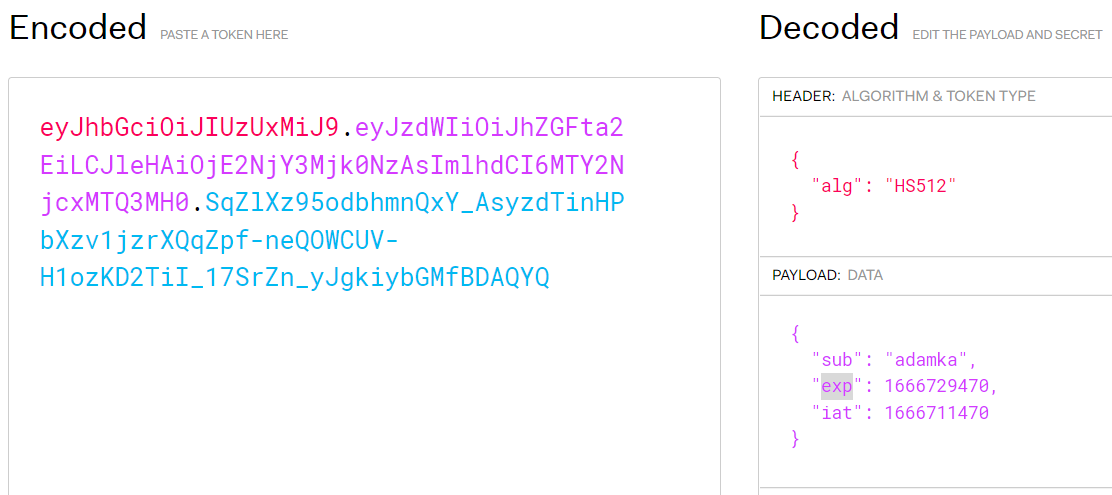
\includegraphics[scale=0.6]{images/jwt.io.png}
\caption{Kódolt és Dekódolt JWT\cite{JWTexample}}
\label{fig:JWT}
\end{figure}